\chapter{Introduction} \label{chap:intro}
%   talk about self-reported pain and intensity estimation
%   why didn't I do any intensity estimation stuff?
%   Regression is difficult??? Classification is a different thing.
%   take about the fact that you are doing one frame and a time and
%   other methods might be better because they can do sequences.

  The human face is most likely one of the most researched objects in image analysis
  and computer vision \cite{S.ZafeiriouA.PapaioannouI.KotsiaM.A.Nicolaou}.
  It has wide ranging applications from Human
  Computer Interaction (expression recognition) to law enforcement (face recognition).
  Its study necessitates the development of a wide range of machine
  learning and computer vision research.

  Facial Action Unit detection FAU \cite{Corneanu2016} is chosen in this work due
  to it's popularity and available benchmarks.
  The Facial Action Coding System (FACS) developed by Ekman and Friesen,
  provides a systematic way to study any kind of facial expression,
  by representing them as a combination of individual facial muscle actions
  known as Action Units (AU). Automating the process of detecting AUs is difficult
  because they have non-linear interactions and often occur in very low intensities.

  There exist many datasets containing images and videos of faces and it is a general
  observation that unlabelled images are far more abundant than labelled ones.
  In particular in the areas of expression recognition where painstaking work
  must be carried out to obtain the ground truth expressions for an image or set of
  frames in a video. This situation is one of the motivations for this project.

  \begin{figure}
   \centering
   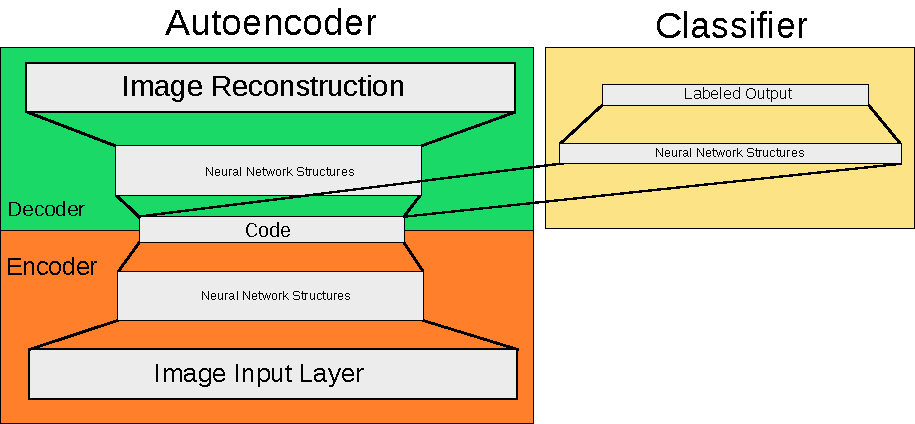
\includegraphics[width=0.8\textwidth]{illustrations/simple_network.pdf}
   \captionof{figure}{General structure of the proposed network. Each rectangle
   represents many layers of neurons and the thin lines represent connections between layers.
   This diagram serves as a very high level description of the structure this project will
   investigate, the boxes in the hidden layers, called neural network structures may contain
   a variety of components including convolutional layers, fully connected layers, dropout layers
   and so on.}
  \end{figure}

  Deep learning is emerging as a powerful tool in modelling a wide range of patterns
  in data, it has been applied to the problem of FAU a number of times and achieved
  good classification rates. One complication which arises when using Deep Neural
  Networks (DNNs) to classify AUs is that many frames are unlabelled (have neutral expressions)
  and hence the standard supervised DNN do not make good use of this information.

  This project takes the DISFA dataset, which is an example of a sparsely labelled dataset, at least
  relative to datasets typically used for Deep Learning tasks, for example MNIST\cite{mnist} which has
  70,000 labelled examples, which all fall into one strictly defined category.

  Further it examines whether
  smoothly transferring between autoencoder training and classifier training can improve
  the ability of the autoencoder to improve classification performance. The constraints mentioned
  include making even low intensity AU occurrences a positive occurrence and not expanding the
  training dataset.

  \section{Potential Applications}
    The ability for a computer vision system to accurately classify actions in a
    human face could have a multitude of application. Human computer interfaces (HCI)
    could benefit from a higher bandwidth interactions between a computer and human, adding
    an extra channel to the typical keyboard and mouse.

  \section{Contributions}
    This work contributes a detailed exploration of how autoencoders and classifiers
    interact in a variety of settings. No substantial performance improvement is noted
    but interesting dynamics are observed. The method of per subject mean and standard
    deviation face normalisaion is put forward as the best way to preprocess images
    for FAU detection.

  \section{Thesis Outline}
    The background relating to FAU detection and relevant deep learning approaches are
    reviewed in chapter
